\documentclass[12pt]{report}

\usepackage{graphics}
\usepackage{epsfig}
\usepackage{times}
\usepackage{amsmath}
\usepackage{framed, color}
\usepackage{fancybox}
\usepackage{graphicx}
\definecolor{shadecolor}{rgb}{0.8,0.8,0.8}

%\usepackage{natbib}
%\usepackage[style=authoryear]{biblatex}
% \addbibresource{mendely.bib} 
% <http://psl.cs.columbia.edu/phdczar/proposal.html>:
%
% The standard departmental thesis proposal format is the following:
%        30 pages
%        12 point type
%        1 inch margins all around = 6.5   inch column
%        (Total:  30 * 6.5   = 195 page-inches)
%
% For letter-size paper: 8.5 in x 11 in
% Latex Origin is 1''/1'', so measurements are relative to this.

\topmargin      0.0in
\headheight     0.0in
\headsep        0.0in
\oddsidemargin  0.0in
\evensidemargin 0.0in
\textheight     9.0in
\textwidth      6.5in

\title{{\bf A Review on Recent Advances in Unsupervised Relation Extraction} \\
\it Term Paper for Recent Advances on Semantics \\ supervised by Prof.Dr.Pinkal}
\author{ {\bf Ehsan Khoddammohammadi}  \\
Faculty of Computational Linguistics \\
Saarland University\\
{\small ehsank@coli.uni-saarland.de}
}
\date{\today}

\begin{document}
\pagestyle{plain}
\pagenumbering{roman}
\maketitle

\pagebreak
\begin{abstract}

The aim of this paper is to review recent and influential methods on
Unsupervised Relation Extraction. In the first chapter, the definition and a general background
for relation extraction task is provided. In the second chapter, four major previous works are
briefly reviewed. And
finally in the last chapter, the paper will be concluded by identifying important aspects and
difficulties of the task and important lessons learned from each of the discussed relation extraction systems.

\end{abstract}

\pagebreak
\tableofcontents
\pagebreak

\cleardoublepage
\pagenumbering{arabic}

\chapter{Introduction}
\label{ch:intro}

\iffalse
This part provides an overall introduction of the unsupervised relation extraction task, including
definition and various formulations of the task.
\fi

Nowadays searching through Internet is the first step we take if we want to get answer to our question.
We convert our questions to sequences of keywords and search engines are trying 
to lead us to web pages where might contain the answer to our questions, they return us a set of related
documents which are sorted by their popularity and similarity of their text to our query.
In this way, users themselves are responsible to find the desired knowledge 
from documents. The next generation search engines should go further than current 
approaches in understanding the meaning of a query and the underlying semantics of documents on 
the web. The next natural improvement is to return a piece of information which directly approaches to 
answer the user question. For this reason, the elements of a query, concepts or entities and 
their relations should be identified and documents ( which might have the answer) should be mapped to the 
same space of entities and relations in order to find the the desired information in the question.

Relation Extraction is the task of detecting and classifying semantic relationship 
between named entities (NE). The goal of this task is to find a triple
of binary relations and their arguments \cite{Androutsopoulos2009}. For instance, we want to induce a
relation like \emph{bornIn} with its arguments which could be for example like this:\emph{ (
bornIn, Beata Nyari, Budapest )}. Applications of such task is numerous
in natural language processing; Question/Answering, machine translation and
text summarization are systems that benefit from relation extraction \cite{Androutsopoulos2009}.

In this task, we are trying to have a model to find paraphrases which means
that we are interested to have all the similar semantically similar relations under
one umbrella. So it is desired to have all different surface realizations of one
relation like \emph{isGivenBirth, isBorn, isFrom} in a same set, namely \emph{bornIn}.

Here, in this paper, we only limit ourselves to review unsupervised relation discovery methods. 
One should mention that there are other approaches for this task based on the extent of resources that they use.
 The different category of approaches is dependent on if they heavily use annotated corpora (supervised learning) or 
 small amount of training data (weakly supervised learning). Here, in contrast, 
 We just discuss methods that do not use annotated resources for inducing the relations and finding the arguments. 



\chapter{Major Recent Works on Unsupervised Relation Extraction}
\label{ch:related}

From a classic method, DIRT \cite{Lin2001}, to very famous frameworks ,
TextRunner\cite{Bankoa} or distant supervision\cite{Mintz2009}, and more recent works e.g. PATTY\cite{Nakashole2012a},
all are examples of several different family of approaches. These methods could
be categorized from different perspectives (1) amount of annotated data they
need (2) if they can only handle a predefined enumeration of entities and re-
lations or are open to any number of relations (3) organization of semantic
interpretation and (4) underlying family of methods they use.
In this section we will review four major works on unsupervised relation discovery.
 We will discuss their formulation of the task, their models
 and the features they incorporate, the model constraints and finally we will take a look at how good a model is performing.


\section{DIRT}
\label{ch:unsupervised}

Lin and Pantel in \cite{Lin2001} proposed an unsupervised method for finding paraphrases from text which  
proved to be very influential and their method, \textbf{DIRT}, has become a classic work in literature.
 In addition
 to this paper we will also review two major improvements to DIRT proposed in \cite{Bhagat2007} and \cite{Pantel2007}.
DIRT tries to cluster semantically equivalent relations based on the similarity of their arguments. Relations
(or inference rules) that DIRT can discover are mostly limited to paraphrases which are a subset of possible types of inference rules.

In this section, first, the key idea of DIRT will be elaborated more and then we will review the algorithm and analyze the observations.
Based on these observations, two other methods, ISP \cite{Pantel2007} and LEDIR \cite{Bhagat2007}, 
which try to address a subset of DIRT's problems, will be discussed.

\subsection{Extended Distributional Hypothesis}
\label{ch:assumption}

Synonymy of words and other semantic relations in word level have been studied very well in literature.
For example Pereira et al. in \cite{Pereira1993} 
cluster similar words which convey a similar meaning. The key assumption in this work and related ones is so called
 \textbf{Distributional Hypothesis} \cite{Harris1981}
 . It tells that words which usually occur in similar context have similar meaning. This idea can be generalized
  to phrases or predicates-arguments. A set of relations or phrases that appear in a similar context
  are semantically equivalent. Lin and Pantel have extended this idea with giving a slightly different notion
   of context. The context that they define in their work is the dependency path between a predicate of
    relation and its arguments. As the Extended Distributional Hypothesis states:
    \begin{shaded}
     If two paths tend to occur in similar contexts, the meaning of the path tend to be similar 
    \end{shaded}
    
      
    In this sense, the task of finding paraphrases or semantically equivalent relations
     can be formulated as \emph{finding paths with similar meaning}. 
     An algorithm to find such a similar path is a topic of the next part.

\subsection{Model Description}
\label{ch:dirt-model} 
DIRT starts with dependency parsing of sentences and continues with pruning of these dependency trees.
It amounts to several conditions on dependency path such as that only nouns will be kept as arguments. 
Additionally, all the function words will be filtered to have the dependency relations that only connect
two content words. Dependency relations with less than a certain number of occurrence will be removed to make the task feasible.
After the pruning phase, a set of binary relations with a list of nouns associated to each of their slots is generated. 
The similarity of relations can be expressed based on similarity of associated list of slot words. Lin and Pantel
have used \emph{pointwise mutual information (pmi)} two measure similarity of slots. 
It measures the independency of two random variables or the amount of
information they contain for each other. The similarity function for relations  is a geometric average
of similarity of correspondent slots.

Instead of clustering of relations which seems to be a natural next phase,
 they maintain a databases of triples (relation and its slots).For each relation queried
  they measure the similarity of relations which share at least one common slot word and then report top-40 of them.
  
\subsection{Evaluation and Analysis}
\label{ch:model} 
  
  Based on what Lin and Pantel have reported in \cite{Lin2001} they extracted 231,000 unique paths from a newspaper corpus.
  They have used a manually generated paraphrases to evaluate their method. For six questions from TREC-8 
  they have generated top-40 paraphrases and then evaluate them manually to report percentage of correctly found paraphrases.
  This approach has a very obvious flaw which is that number of returned paraphrases is fixed. Clustering has this 
  advantage that each cluster of relations can have arbitrary number of paraphrases.
  Average accuracy for these six questions is 50.3\% and no paraphrases have been found for one of the questions.
  The recall can't be measured easily since many correctly found paraphrases by DIRT are not discovered by humans.
  
  Beside the problem of having fixed number of returned paraphrases, there are three other major 
  problems after observing the results of DIRT which two of them will be addressed by Pantel et al. and
  will be discussed in the next parts. These problems are:
  
  \begin{enumerate}
    \item Antonymy of relations can not be captured with DIRT and antonym relations will be returned as similar relations. After more than
    a decade, it is still an open problem
    \item DIRT results are very noisy in a sense that it doesn't induce the type of arguments.
    \item DIRT results or paraphrases are always considered as bi-directional. Relation \emph{A} implies relation \emph{B} and vice versa.
    This assumption doesn't hold for many instances and needs to be regarded in the model.
  \end{enumerate}
  
In the next two sections ISP and LEDIR methods will be covered as proposed improvements to DIRT to filter erroneous relations.
   

\subsection{Inference Selectional Preferences}
\label{ch:sel-pref} 

Selectional preference of a predicate is the constraint that it puts over the class of words can be used as its arguments.
For example: \emph{x drives y} has a selectional preference on the second argument for motorized 
vehicles with more than two wheels and \emph {x rides y}
has a preference for vehicles or animals which rider is positioned astride \cite{Mechura2008} .

In order to model this type of constraint on discovery of paraphrases, Pantel et al. \cite{Pantel2007} have proposed that
relations which are similar but are not sharing a same class of arguments should be filtered out. For each relation, 
they compute a distribution of possible semantic classes for its arguments. For two equivalent relations, they will be kept
if this distribution is similar for both.Yao et al. \cite{Yao2011} also incorporate selectional preferences to their model and which we
will see in detailed in the last section.

Two models are proposed to compute this distribution. The first one, the distribution is computed jointly for both of arguments
and the second one two different distributions are computed for each argument. The computation is just a simple count.

The question that naturally arises is that how one can obtain these semantic classes? The answer is that
they are obtainable from lexical resources such as WordNet or they can be induced by clustering words.
The authors have used both methods. As the first approach, they have used top level nodes in WordNet and all their successors together
as semantic classes. They have also used CBC clustering algorithm \cite{Pantel2002} to induce semantic classes. 
In \cite{Brown1992} and \cite{Lin2009} a similar approach but with different clustering algorithms has been chosen 
and the later is the current state-of-the-art method. 

After computing selectional preferences for each relation, those relations which don't have similar selectional preference
distribution will be considered as nonequivalent. The plausibility of an inference rule which contains two relations is
discussed in detailed in \cite{Bhagat2007} and \cite{Kotlerman2010} .

Inducing word clusters and using independent selectional preferences distributions has been shown to outperform other models
and have the highest increase of accuracy compare to DIRT.     

\subsection{Direction of Inference Rules}
\label{ch:improve}
So far all the similar relations are considered to be paraphrases and they have bi-directional semantic equivalency relation.

Since this assumption doesn't hold for all the inference rules that are discovered by DIRT, Pantel et al. pushed their model
another step further to find the direction of implications among relations, in addition to just find equivalent relations.

They have used the results from DIRT and ISP to find out which direction holds for an implication over two relations.
having $relation_i \iff relation_j$ they want to examine if it holds or either of $relation_i \implies relation_j$
or $relation_j \implies relation_i$ is the correct rule. 

the key assumption in \cite{Bhagat2007} is that the direction is most likely from a specific relation to a more general relation.
By specific relation they mean a relation that has a narrow set of semantic classes and selectional preferences and 
a general relation is a relation with broader semantic classes. Number of acceptable semantic classes for each relation is a 
good measure for such purpose. If this number is greater for the antecedent then the direction is right otherwise it should be flipped.
A similar approach has been used in \cite{Kotlerman2010} which additionally confirm the results of this work.

In the next section we will review a method which operates in web-scale and extract relations with bootstrapping.




\section{TextRunner}
\label{ch:unsupervised}

TextRunner is the first system that addresses open domain relation extraction in web-scale \cite{Yates2007}. In this section
 we will describe the architecture of TextRunner and then we will review two main elements of this system, \emph{Learner} and
  \emph{Extractor}, in more details and shortly we will comment on the third element \emph{Assessor}.
 
\subsection{TextRunner Architecture}
\label{ch:arch}

Original TextRunner paper proposed four elements for its architecture:
\begin{itemize}
  \item Learner
  \item Extractor
  \item Assessor
  \item Query Processor
\end{itemize}

The last sub-system has no major role in relation extraction so we put our focus on the first three elements.

\subsection{Model Description}
\label{ch:model}

TextRunner avoids using parsing for large-scale and inhomogeneous corpus like web. \emph{Learner} sub-system is responsible
 for providing a substitution or an approximation for syntactic parsing which, called as extractor by the authors.
  The approach that they follow in \cite{Yates2007}
  is that they use a small corpus to train a  relation classifier and this classifer will be applied to a much bigger web corpus.
   After parsing the small corpus, authors have used a set of predefined heuristics just based on POS tags and syntactic role 
   of words to generate positive ad negative relation examples. The heuristics were designed as prototypes of syntactic behavior
   of general relations and they are not dependent on any certain type of relation. 
   For example:   $E_1 \;\; Verb \;\; E_2$ as template of \emph{X created Y} or 
   $ E_1 \; \; NP \;  Prep \; \; E_2$ for \emph{X is birthplace of Y} are such heuristics.\\
   
   
    
    A Naive Bayes classifier is self-trained on this small dataset, it 
   starts with small seed of relations for training then it labels more instances in the corpus. This classifier will be used as
    \emph{Extractor}
   in the next phase. This classifier is not relying on any lexical or relation-specific features, hence it can operate 
   in open domain like web \cite{Banko2009}. In the extraction phase, a maximum-entropy classifer was used to find entities and then by 
   using the extractor learned from the previous phase, they recognize explicit relations among named entities.
   
   These extracted relations and named entities contain many redundant or equivalent relations. The role of \emph{Assessor}
    is to find equivalent relations. It starts with normalization of relations and entities and then based on string-similarity
     and shared relational attributes it finds explicitly equivalent relations, it should be mentioned that 
     this approach differs from DIRT which finds semantically equivalent relations.
     
      
     
\subsection{Evaluation}
\label{ch:eval}
     
     TextRunner is evaluated against a manually tagged dataset of 500 sentences. While the precision is in 
      the accepted level, 86.6\%, recall is low (23.2\%). The recall has been improved by using a \emph{Conditional Random Field}
       \cite{Banko2009} as classifier instead of Naive Bayes. The model precision is slightly improved by using a CRF for about 2\%
        but we see a tremendous increase in recall which levels to 45.2\% . 
 
TextRunner suffers from using very shallow features. Its ability to find relations is limited to explicitly mentioned
 relations and it can only find them if they occur in a sentence. In the next part we will review a model 
 which does not suffer from these disadvantages due to its deeper semantic analysis. 
 

\section{USP}
\label{ch:unsupervised}

In this section we will review the first unsupervised semantic parsing method which proposed by Poon and Domingos \cite{Poon2009},
we will first define what is semantic parsing and after describing the method in \cite{Poon2009} we show its application for relation extraction.
In the evaluation subsection we will compare this model to its related models and analyze its advantages and disadvantages.

\subsection{Semantic Parsing}
\label{ch:definition}

Semantic parsing is mapping a sentence to its formal meaning representation \cite{Poon2009}
The aim is to represent a natural language text with first-order logic. One can derive a semantic parse of a sentence
by starting from a lexicon of atomic formulas and combining each fragment to build a composition of 
formulas combined with quantifiers and logical connectives. In \cite{Poon2009} 
the lexicon will be induced from a raw corpus. It is in contrast to traditional means of semantic parsing with manually
  produced lexicons.
  
  The main challenge in unsupervised semantic parsing is that for a single semantic representation there could be
  several syntactic realizations or even harder, different surface representations. For example, all of the
   sentences below has a same semantic representation:
   \begin{itemize}
     \item Microsoft buys Skype
     \item Microsoft acquires the VoIP company Skype
     \item Skype is acquired by Microsoft Corporation
     \item The Redmond software giant buys Skype
     \item Microsoft’s purchase of Skype,\ldots
   \end{itemize}  
  
   A simple lexicon to represent all of the examples above is:
  
   $$ BUY(n_1)$$
   $$ \lambda x_2.BUYER(n_1 , x_2) \; \;  \lambda x_3.BOUGHT(n_1 , x_3) $$
   $$ MICROSOFT(n_2) \; \; SKYPE(n_3)$$
   
   Having a corpus of sentences in natural language, USP \cite{Poon2009}
    will induce such a lexicon and will also extract a formal representation for each sentence. In the next 
    subsection we will review the necessary steps toward this goal.
\subsection{Model Description}
\label{ch:model}
In this section we will first identify the three key ideas that the model is built upon them and then 
we will describe the necessary steps toward unsupervised semantic parsing.

Three observations are made by the authors which is crucial to understand the model assumptions:

\begin{enumerate}
  \item Different syntactic variations of predicates and constants can be clustered together to express
   a same meaning. This can be learned from a raw corpus, in contrast to supervised methods which use meaning annotation of text.
   \item Not only fixed elements in a relation can be clustered together but also arbitrary forms with same sub-forms to co-occurred forms 
   can be put in a cluster. In this way the meaning composition will be learned through clustering of the forms.
   \item Learning syntax and semantics jointly is a complex problem. Authors have shown that translating a syntactic analysis
   to semantic parse has superior performance over joint learning of syntax and semantics. In this way, a model can be built on the shoulder
   of state-of-the-art syntactic parsers.
   
\end{enumerate}

Based on these assumptions, they propose a method to model joint probability of the dependency tree
and its meaning representation. Markov Logic Networks (MLN) \cite{Richardson2006} is used to represent the meaning of a sentence.
For each sentence we will have an undirected graphical model (Markov network) which each nodes corresponds to atoms
and cliques correspond to first-order clauses. The best meaning representation is the one which 
maximizes the probability of the observed dependency \cite{Titov2011}.
These are the major steps of the USP system:
\begin{description}
  \item[Dependency Parsing] \hfill \\
  the authors believe that dependency parsing is a better starting point that phrase-structure parsing, since it expresses
   the relation-argument structure at the lexical level. They have used Minipar \cite{Lin2002} to make the results more comparable with previous
   methods, e.g. DIRT.
  \item[Converting Dependency Trees into Quasi-Logical Forms] \hfill \\
  Extracting lambda forms and atoms (lexical entries) is done by a deterministic procedure. 
  Arguments of a dependency path will be converted to atoms, their predicate consists of the lemma and their part-of-speech tags.
  Each edge from the head to arguments will be a predicate labeled as type of the dependency path.
  This predicate together with two lambda function for each argument form a QLF. In this QLF, only one constant can be presented.
  
  \item[Clustering Lambda-Forms] \hfill \\
  It starts from atom levels and cluster them based on their relation, then it recursively clusters larger formula
  based on their subformula lambda forms. The composition of meaning of any formula can be obtained by applying
  \emph{lambda reduction} and substituting constants with lambda variables. At the end we will have a clustering
  of lambda forms which each cluster contains a set of semantically equivalent lambda forms. this solves
   the problem of having different syntactic realizations with a same meaning.
  
  \item[Creating a Markov Logic Network] \hfill \\
  Each atom can be modeled as a node and each first-order clause can be modeled as a feature. This is still not a complete Markov Logical
  Network since this model needs a weighting for features.Thus, the weight of feature is defined as a weight of
  its correspondent clause. A log-linear distribution 
  $$ P(x) = \frac{1}{Z}\exp{\Sigma_i{(w_i n_i (x))}} $$
  is used to model the probability of each clique (configuration of nodes and features).
  $Z$ is a normalization factor which its computation is infeasible. $w_i$ is the weight of $i$th formula.
  $n_i$ is number of satisfied atoms and formulas that appeared in the sentence. 
   
  \item[Learning the weights of MLN] \hfill \\
  Given the dependency parse and QLF forms, weights can be learned from data such as the log-likelihood
  of having QLFs given the dependency trees will be maximized. The form of likelihood is:
  $$ L_{\theta}(QLF) = \log{\Sigma_L{P_\theta{(QLF, L)}}}$$ where $L$ is a semantic parse.
  
  Since the summation of all possible semantic parses is infeasible, a set of additional constraints on the form
  of clauses and also a prior over weights are added to model to make the learning feasible. Their algorithm
  merges any possible two clusters to form a bigger cluster or create a new cluster if either increases the likelihood.
  \item[Finding the Best Semantic Parse] \hfill \\
  A semantic parse is a partition of atoms of a QLF, assignment of its head and argument form to a cluster. 
  This can be seen as a structure prediction problem. Given the described MLN and its parameters, inference can
   be done by finding a Maximum A Posterior solution. An exact solution needs a summing over all possible syntactic realizations and
   possible dependency parses, therefor a greedy algorithm to search for a good solution is proposed 
   by the authors.   
\end{description}

\subsection {Evaluation}
\label{ch:evaluation}
Since USP is the first system for unsupervised semantic parsing, it is compared against other models in a Question/Answering task.
GENIA is an Q/A annotated dataset in medical domain and USP has been shown to find the answers with 88\% precision
which is about 10\% higher than TextRunner and more than 30\% better than DIRT. It is worthwhile to mention that
GENIA is a rather small dataset.

There are two major problems observed by the authors themselves and others for USP.
\begin{itemize}
 \item Same as the other models that we have already seen,
 it doesn't address the separation of antonym relations
 \item It is mentioned in \cite{Yao2011} and \cite{Titov2011}
  that USP suffers from using a large memory and therefore low ability to scale to bigger dataset. 
 \end{itemize}
 Two modifications for USP runtime is proposed in \cite{Poon2013} and \cite{Titov2011}.
  In \cite{Titov2011}
   it is proposed to use directed graphical models instead of undirected graphs(MLN) to increase the learning and inference speed.
  The result is slightly worse than the original model but it performs faster than USP.
  In \cite{Poon2013} 
  a new representation of the model is given in the framework of deep learning which yields 
  the same performance but with faster learning algorithm.
  
  In the next section we will see another model which shows improvement to DIRT, TextRunner and USP 
  and is much more scalable than the former.
     

\section{Rel-LDA \& Type-LDA}
\label{ch:unsupervised}

In this section we will review the method proposed for relation discovery  by Yao et. al. \cite{Riedel2013}  
The method they  proposed is an unsupervised method using generative models which is based on 
modification of well-known model, Latent Dirichlet Allocation. 
They have invented three similar models which we will go through them in following. 
We elaborate on input of the three models and then we describe their generative story 
and at the end we will finish this part by discussing about  model evaluation.

\subsection{Input format and preprocessing}
\label{ch:input}
Authors have chosen a subset of New York Times articles from year 2000 to 2007 which some of its parts with
abnormal style of writing like obituary content are filtered out.
They have done several preprocessing steps:
\begin{enumerate}
\item Tokenization
\item Sentence split
\item POS tagging %(?? all last three steps with Stanford tools)
\item Named entity tagging % ( ?? Finkel2005)
\item Dependency parsing %(??MaltParser)
\end{enumerate}
Among all dependency paths they are just interested in those which link two named entities.
 Authors assume that realization of one relation is available in this 
 path most likely as a verb which relates two mentioned named entities. These types of 
 paths are collected and based on some conditions that we have already discussed in Section ~\ref{ch:dirt-model} ,
  non-important links are filtered out.
 Finally in this phase, 2.5 million dependency paths were collected 
 which will serve as an input to the models that we describe in the next subsection.


\subsection {Model Description}
\label{ch:model}
All the three models in this work are generative models. Generative models are jointly modeling hidden variables and observable variables and 
are in contrast to discriminative models. For more information on generative models please see \cite{Murphy2012}.\\


\textbf{Rel-LDA} is the first model proposed in \cite{Riedel2013}. 
In this model, features, $f$, are generated from a distribution , $\Phi_{rf}$. Each type
 of relation is represented with a binary indicator variable, $r$. Each document is a mixture of few relations
  and relations are generated from a multinomial distribution $\Theta_{doc}$. $\Theta_{doc}$ is a distribution
  of relations for a specific document and can be shown as $P(r|doc)$. By choosing a right prior distribution for $\Theta$
   and $\Phi$ we can impose an assumption that any document contains a few number of relation types. 
   Another advantage of having prior is that it helps to avoid overfitting. Dirichlet prior with small parameter $\alpha$ is 
   chosen for this purpose in the paper. For more on the role of priors and specially Dirichlet prior
    please read \cite{Teh2007} and \cite{Gershman2012} .
    Rel-LDA is described with a graphical model 
     \begin{figure}[h!]
  \caption{Rel-LDA}
  \centering
    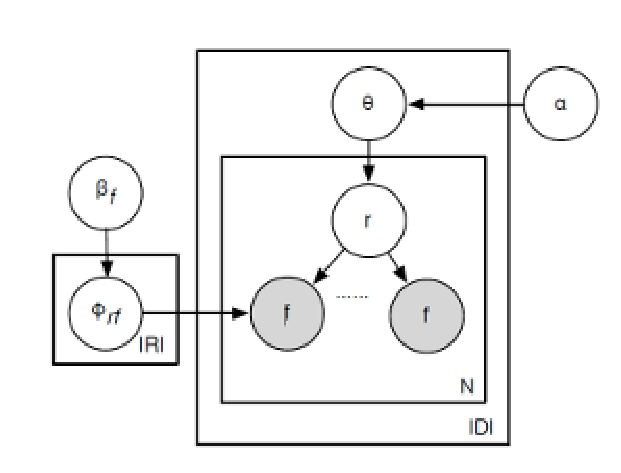
\includegraphics[width=0.5\textwidth]{rel-lda.eps}
    \label{fig:rel-lda}
\end{figure} in Figure ~\ref{fig:rel-lda} .
     
    Shaded circles are showing the observable variables and other circles are hidden variables except 
    the priors which are set by ourselves. The direction of arrow shows the dependency in this sense 
    that destination node (variable) is dependent on source node.
      
    Features or observable variables in Rel-LDA are:
    \begin{itemize}
      \item The dependency path
      \item Source of the path (the first named entity)
      \item Destination of the path (the second named entity)
    \end{itemize}
   	
   	An exact sampling method called \emph{variational inference} is used by authors to compute 
   	the posterior distribution of the model, $P(r|f)$.
   	After learning, we will have clusters of relation types which each instance of a specific cluster 
   	is a relation that is supposed to be semantically equivalent to the other members of this cluster.
   	\\
   	
   	In the second model, \textbf{Rel-LDA1},The only difference is that  more features are used in the learning procedure.
   	 The idea is that using more features could be useful as tie-breakers and also discriminators between instances
   	  to make new clusters. With direct reference to the paper, the authors believe that more features 
   	  lead to better refinement of clusters. We will see later that this assumption holds in practice.
   	   The new features that they have introduced in this new model are:
   	   \begin{itemize}
   	     \item Trigger: Any word in a dependency path except than stop words. 
   	     \item Part of speech sequence: The sequence of POS tags of a dependency path. 
   	     \item Named entity pair: The type of source and destination named entity.
   	     \item Syntactic pair: The type of dependency edges connecting source and destination to the head.
   	   \end{itemize}   
   
 Among all the newly introduced features, NE pair is the most interesting one which leads to a 
 significant observation that the third model will try to address that. Authors observed that 
 Rel-LDA will put these three relations in one cluster because the second argument of all of them is location:
 
 \begin{enumerate}
   \item \emph{ X was born in Y}
   \item \emph{ X lives in Y}
   \item \emph{ X, a company in Y}
 \end{enumerate}
 
 While the first argument in the first two relations refers to a PER, the first argument of the 
 third relation is an instance of ORG type. By using NER pairs as feature we can split this cluster 
 to two clusters with respect to basic types of NE in relations arguments. 
 This observation leads us to invest more on type identification of arguments to have more pure 
 clusters and is the main focus of the third model, \textbf{Type-LDA}.
 
 
 Selectional preferences of a relation are constraint over possible arguments for the relation.
  Basically, any relation only accepts a few number of entity types and this could be an important constraint
   for inducing relations. Relations of each cluster should have similar selectional preferences and
    accept same entity types. Type-LDA is proposed for this reason, it will induce entity types 
    and relation clusters jointly to benefit more from selectional preferences of relations. 
    As we have already mentioned in Section ~\ref{ch:sel-pref},
     this idea have been used in \cite{Pantel2007} .
    
    The generative model is modified in a way that features of arguments (source and destination)
    will be generated from two new distributions, $T_1$ \& $T_2$ which are modeling entity types. The graphical model
    is shown in
     \begin{figure}[h!]
  \caption{Type-LDA}
  \centering
    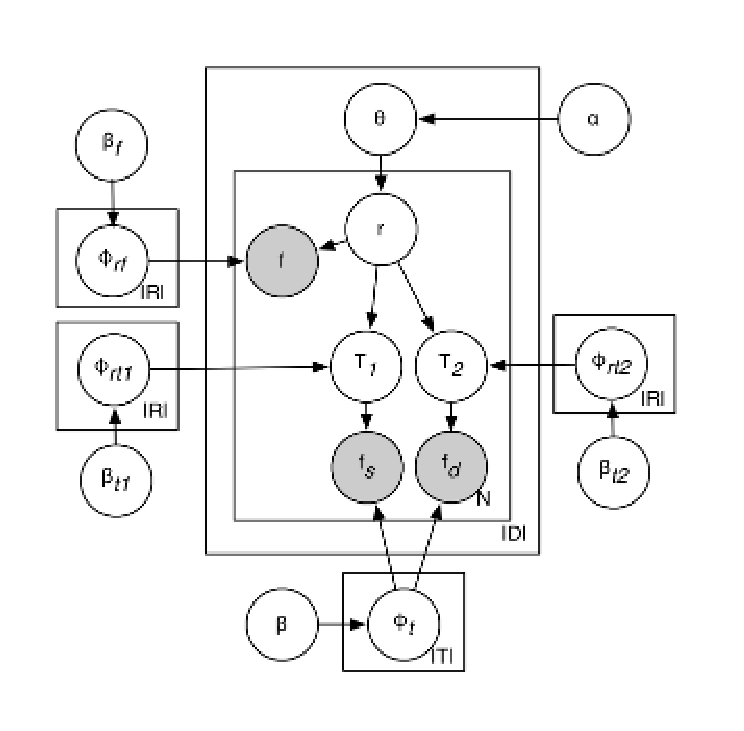
\includegraphics[width=0.5\textwidth]{type-lda.eps}
    \label{fig:type-lda}
\end{figure} 
Figure ~\ref{fig:type-lda} .
    This model not only clusters relations but also clusters entities to entity clusters.
    
    For their experiments on all three models they have set the number of relation clusters to 100 and for Type-LDA they used 
     50 entity clusters. Choosing other numbers of relation clusters in the range of 50 to 200 is shown to be not very significant.
    
\subsection {Evaluation}
\label{ch:evaluation}

\iffalse Yao et al. have evaluated their models in different settings.  Their comparison against Mintz et al.?? previous work
 will be mentioned in the next chapter which is dedicated to distant supervision. \fi They have used human judgments 
 to measure their models precision. Humans are asked to label 50 instances in each relation cluster and in order to measure
 the recall, induced relations are compared against Freebase. Rel-LDA1 and Type-LDA which are using selectional preferences features
  are performing better than Rel-LDA. Rel-LDA1 is shown to have the best precision among other models. 
  Rel-LDA and Type-LDA have been also compared against
  USP and have been shown to have superior performance both in scalability and F-measure. 
 
 Like most of the other models, antonymy is not handled in their model and therefor for example they have
 \emph{X was born in Y} and \emph{X die in Y} in one cluster.
 
 Entity clusters also sometimes suffer from high-frequency or low-frequency words and for example, `New York`
 , is in the same cluster as other publications like `New York Times`, `Vanity Fair` and \ldots
 
 Yao et al. have shown that they have induced relations in different granularity from Freebase and reported some relations
 which are not mentioned in Freebase but positively hold. For example, Freebase relation \emph{worksFor}
  is subsumed with more relations each indicates a different role of employment relation. \emph{leaderOf}
   and \emph{editorOf} are such examples. This will boost the idea of inducing hierarchical 
   relations which will be discussed more in the last chapter. A similar approach which tries to induce
    hierarchical structures is \cite{Alfonseca2012} .
 
 
\iffalse
\chapter{Weakly Supervised on Relation Extraction Task}
\label{ch:related}

\section{Distant Supervision}
\label{ch:weakly supervised}


The content of \cite{Huang2012} your proposal. Each topic occupies one section, each
with their own conclusion and future work.
\fi

\chapter{Conclusion}
\label{ch:conclusion}

\section{Analysis}
\label{ch:conclusion}

Based on what we have seen in recent works, we can now give a list of vital
attributes that a state-of-the-art model for extracting relations from open text
should be able to carry out. The author will use these facts to suggest a list of possible improvements
in the next section. Modeling all of
these factors in a joint model is the necessary step to push forward the previous
works.

\begin{description}
  
  \item[The number of relations and entities is an unknown parameter.] \hfill \\
  The model can not be confined to a limited set of relations or entities. Being able to extract relations in
  open domain text is the first and (most likely) a trivial attribute of the model. More non-trivial feature
  of the model should be its ability to extract as many relations as there are in text. 
  Giving this freedom
  about the model complexity to have no assumption about the exact number of entities and relations
  is suggested by the applicant to be beneficial 
   and is also supported in the literature.
   \cite{Mintz2009} \cite{Yates2007}  

  \item[Relations may not be expressed explicitly in text.] \hfill \\
  Relation extraction task is definitely more than finding paraphrases. The model should be able to handle
  long-distance relations among entities as well as hidden semantic indications of a relation. \cite{Poon2009}
  


  \item[Relations and entities have their inner organization and types.] \hfill \\
  It is shown by several recent works that relations of relations play a substantial role in identifying
  relations. Relations and entities belong to a hierarchy of types and therefore the constraints they put on each other
  should be learned as well.\cite{Yao2011} \cite{Alfonseca2012} \cite{Nakashole2012a}

  \item[Using KB is necessary but not enough.] \hfill \\
  There are more relations among entities than what is collected in 
  Knowledge Bases e.g. Freebase. At the same time, it is statistically shown that a supervision
  from such resources strongly contributes to convergence of any model to a better 
  objective configurations.\cite{Yao2011} \cite{Mintz2009}

  \item[Relations and entities are sharing information within each other.] \hfill \\
  Relations and entities should be learned jointly since they share same explanatory factors (hidden variables)
  . Meaning of an entity can be learned from its relation to other entities and same argument holds among relations.
  Basically, the model should be able to carry out multi-task learning. \cite{Yao2011} 
    
\end{description}


\section{Summary}
\label{ch:conclusion}

In this paper, we reviewed four influential works on \textbf{Unsupervised Relation Extraction}:
\begin{enumerate}
  \item DIRT
  \item TextRunner
  \item USP
  \item Rel-LDA \& Type-LDA
\end{enumerate}

We described each model and analyzed the strength and weakness of them. We also showed some improvements over these
 methods in literature. At the end, we highlighted main aspects of the task that each model tried to address a subset of them.
 

%\subsection{Plan for completion of the research}

%Table \ref{tab:plan} shows my plan for completion of the research.

%\begin{table}[hc]
%\begin{small}
%\begin{center}
%\begin{tabular}{lll}
%Timeline & Work & Progress\\
%\hline
%          & XXXXXXXXXXXXXXXXXXXXXXXXXXXXXXXXXXXXX & completed\\
%Nov. xxxx & XXXXXXXXXXXXXXXXXXXXXXXXXXX & ongoing\\
%Jan. xxxx & Thesis writting & \\
%Feb. xxxx & Thesis defense & \\
%\end{tabular}
%\end{center}
%\end{small}
%\caption{Plan for completion of my research}
%\label{tab:plan}
%\end{table}



\pagebreak

\begin{footnotesize}
\bibliographystyle{plain}
%\bibliographystyle{agsm}
\bibliography{mendely.bib}
%\printbibliography
\end{footnotesize}

\end{document}


